    \documentclass{beamer}
    %\documentclass[trans]{beamer}
    %\documentclass[handout]{beamer}
    

    \mode<handout>
    {
      \usepackage{pgfpages}
      \pgfpagesuselayout{2 on 1}[a4paper,border shrink=5mm]
    }
    
    \usetheme{Berlin}
        \defbeamertemplate*{footline}{infolines theme}
{
  \leavevmode%
  \hbox{%
  \begin{beamercolorbox}[wd=.333333\paperwidth,ht=2.25ex,dp=1ex,center]{author in head/foot}%
    \usebeamerfont{author in head/foot}\insertshortauthor
  \end{beamercolorbox}%
  \begin{beamercolorbox}[wd=.333333\paperwidth,ht=2.25ex,dp=1ex,center]{title in head/foot}%
    \usebeamerfont{title in head/foot}\insertshorttitle
  \end{beamercolorbox}%
  \begin{beamercolorbox}[wd=.333333\paperwidth,ht=2.25ex,dp=1ex,right]{date in head/foot}%
    \usebeamerfont{date in head/foot}\insertshortdate{}\hspace*{2em}
    \insertframenumber{} / \inserttotalframenumber\hspace*{2ex} 
  \end{beamercolorbox}}%
  \vskip0pt%
}
    
    \useoutertheme{infolines}
    % There are many different themes available for Beamer. A comprehensive
    % list with examples is given here:
    % http://deic.uab.es/~iblanes/beamer_gallery/index_by_theme.html
    % You can uncomment the themes below if you would like to use a different
    % one:
    %\usetheme{AnnArbor}
    %\usetheme{Antibes}
    %\usetheme{Bergen}
    %\usetheme{Berkeley}
    %\usetheme{Berlin}
    %\usetheme{Boadilla}
    %\usetheme{boxes}
    %\usetheme{CambridgeUS}
    %\usetheme{Copenhagen}
    %\usetheme{Darmstadt}
    %\usetheme{default}
    %\usetheme{Frankfurt}
    %\usetheme{Goettingen}
    %\usetheme{Hannover}
    %\usetheme{Ilmenau}
    %\usetheme{JuanLesPins}
    %\usetheme{Luebeck}
    %\usetheme{Madrid}
    %\usetheme{Malmoe}
    %\usetheme{Montpellier}
    %\usetheme{PaloAlto}
    %\usetheme{Pittsburgh}
    %\usetheme{Rochester}
    %\usetheme{Singapore}
    %\usetheme{Szeged}
    %\usetheme{Warsaw}
    
    
    \usepackage{natbib,bibentry}
    \usepackage[utf8]{inputenc}
    \usepackage[english]{babel}
    \usepackage[T1]{fontenc}
    \usepackage{float}
    \usepackage{amsmath}
    \usepackage{graphicx}
    \usepackage{amssymb}
    \usepackage{amsthm}
    \usepackage{float}
    \usepackage{caption}
    \usepackage{enumitem}
    \usepackage{minted}
    \usepackage{parcolumns}
    \usepackage[normalem]{ulem}
    \usepackage{tikz}
     \usetikzlibrary{shapes,snakes, fit}
    \usetikzlibrary{scopes,backgrounds}
    \usetikzlibrary{calc, positioning, matrix,arrows}
    
    
    \title{Functional Game Programming}
    
    % A subtitle is optional and this may be deleted
    %\subtitle{}
    
    \author{David Kr\"{a}utmann, Philip Kindermann}
    % - Give the names in the same order as the appear in the paper.
    % - Use the \inst{?} command only if the authors have different
    %   affiliation.
    
    \institute{RWTH Aachen}
    % - Either use conference name or its abbreviation.
    % - Not really informative to the audience, more for people (including
    %   yourself) who are reading the slides online
    
    % This is only inserted into the PDF information catalog. Can be left
    % out. 
    
    % If you have a file called "university-logo-filename.xxx", where xxx
    % is a graphic format that can be processed by latex or pdflatex,
    % resp., then you can add a logo as follows:
    
    % \pgfdeclareimage[height=0.5cm]{university-logo}{university-logo-filename}
    % \logo{\pgfuseimage{university-logo}}
    % Let's get started
    
    %tikz
    \tikzset{button/.style={draw=red, circle, minimum height=4em}}
    \tikzset{block/.style={draw=black, rectangle, minimum width=6em}}
    \tikzset{outblock/.style={draw=blue, rectangle split, rectangle split parts=2, minimum width=4em}}
\tikzset{pure function/.style={draw=black, circle, minimum width=3em}}
\tikzset{signal function/.style={draw=black, rectangle, minimum width=3em}}
\tikzset{signal function with state/.style={draw=black, rectangle split, rectangle split parts = 2, rectangle split draw splits = false, minimum width=6em}}
    \tikzset{highlight/.style={draw=blue, text=blue}}
    
    \begin{document}
    
    \begin{frame}
      \titlepage
    \end{frame}
    
\begin{frame}{Outline}
  \tableofcontents
  % You might wish to add the option [pausesections]
\end{frame}
    
    \section{Motivation for FRP}
    \begin{frame}{Motivation for FRP}
        \begin{itemize}
            \item Real-time programming is imperative
            \begin{figure}[ht]
            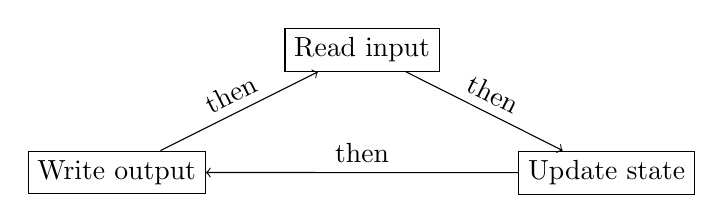
\begin{tikzpicture}
            \node[rectangle,draw] (read) {Read input};
            \node[rectangle,draw,below right=of read] (update) {Update state};
            \node[rectangle,draw, below left=of read] (write) {Write output};
            \path[->, every node/.style={sloped,anchor=south,auto=false}]
            (read) edge  node {then} (update)
            (update) edge node {then} (write)
            (write) edge node {then} (read);
            \end{tikzpicture}
            \end{figure}
            \item Describe what we \emph{want}
        \end{itemize}
    \end{frame}
    
\begin{frame}[fragile]{Motivation for FRP}
        \begin{itemize}
            \item<+-> Benefits of functional programming:
            \item<+-> Expressive code
            \begin{minted}[breaklines]{haskell}
within ball paddle = near paddle.x 8 ball.x && near paddle.y 20 ball.y
            \end{minted}
            \item<+-> More code reuse
        \end{itemize}
% do not indent this when using fragile for minted
\end{frame}
    
    \section{Functional Reactive Programming}
    \begin{frame}{What is FRP?}
        \begin{itemize}
            \item<+-> Model time-varying values
            \item<+-> In first-class datatypes
        \end{itemize}
    \end{frame}
    
    \begin{frame}{Approaches to FRP}
            \begin{itemize}
            \item Classic FRP (Fran, reactive) 
            \item Arrow-based FRP (Yampa, Netwire, Elm)
        \end{itemize}
    \end{frame}
    
    \subsection{Classic FRP}
    
\begin{frame}[fragile]{Behaviours}
\begin{itemize}
\item First-class behaviours:
\inputminted{haskell}{Behaviour.hs}
\item Created by \emph{primitves} or composing other Behaviours
\begin{minted}[breaklines]{haskell}
time :: Behaviour Time
time = Behaviour id

position :: [Time] -> Behaviour Velocity 
         -> Behaviour Position
position s v  = integral 0 s v
\end{minted}
\end{itemize}

\end{frame}

\begin{frame}[fragile]{Events}
\begin{itemize}
\item Events model discrete phenomena
\inputminted{haskell}{Event.hs}
\item Example: \mintinline{haskell}{keysPressed :: Event [Key]}
\begin{minted}[breaklines]{haskell}
occurrences keysPressed = [(After 0, [KeyA, KeyW]), (After 0.5, [])]
\end{minted}
\end{itemize}
\end{frame}

    \subsection{Arrow-based FRP}
    \begin{frame}{Arrow-based FRP}
    \begin{itemize}
    \item<+-> Abstraction of classic FRP
    \item<.-> Core concept: Replace functions with \emph{signal functions}
    \item<+-> Signal: time-changing value
    \item<.> Signal function: Function on signals + state
    \begin{figure}[ht]
\centering
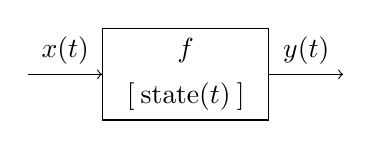
\begin{tikzpicture}[node distance=2cm]
\node[signal function with state, minimum width=6em] (arrf) {$f$ \nodepart{second} $[\: \operatorname{state}(t) \: ]$};
\coordinate[left of=arrf] (in);
\coordinate[right of=arrf] (out);
\draw [->] (in) to node[auto] {$x(t)$} (arrf);
\draw [->] (arrf) to node[auto] {$y(t)$} (out);
\end{tikzpicture}
\end{figure}
    \item<.> State represents input history $\rightarrow$ composable
    \end{itemize}
    \end{frame}
    
    \subsection{Signal functions}
\begin{frame}[fragile]{Signal functions}
        \begin{itemize}
        \item Signal functions either inhibit or produce
        \item 
\begin{minted}{haskell}
data Maybe a = Just a | Nothing

data SF s a b 
  = SFArr (a -> b)
\end{minted} 
    \item Any pure function is a signal function
    \mint{haskell}{arr :: (a -> b) -> SF s a b}
    \item Necessarily stateless: \mint{haskell}{arr = SFArr}
    \end{itemize}
\end{frame}

\begin{frame}[fragile]{Signal functions}
        \begin{itemize}
        \item Signal functions either inhibit or produce
        \item 
\begin{minted}{haskell}
data Maybe a = Just a | Nothing

data SF s a b 
  = SFArr (a -> b)
  | SFPure (s -> Maybe a -> (Maybe b, SF s a b))
  | ...
\end{minted}
\end{itemize}
\end{frame}

    \begin{frame}{Composition}
    \begin{itemize}
    \item Signal functions can be composed
    \begin{figure}[ht]
    \centering
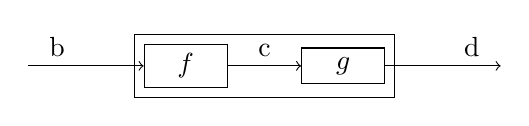
\begin{tikzpicture}[node distance=2cm]
\node[signal function, minimum width=3em] (f) {$f$};
\node[signal function, minimum width=3em, right of=f] (g) {$g$};
\node[signal function, fit=(f) (g), minimum width=6em] (arrf) {};
\coordinate[left of=f] (in);
\coordinate[right of=g] (out);
\draw [->, near start] (in) to node[auto] {b} (f);
\draw [->] (f) to node[auto] {c} (g);
\draw [->, near end] (g) to node[auto] {d} (out);
\end{tikzpicture}
\caption*{$f \ggg g$}
\end{figure}
\item For stateless SF:
\mint{haskell}{SFArr f >>> SFArr g = SFArr (g . f)}
\end{itemize}
\end{frame}
\begin{frame}[fragile]{Partial application}
\begin{itemize}
    \item Signal functions can be applied to a part of the input
    \begin{figure}\centering 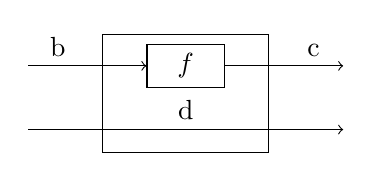
\begin{tikzpicture}[node distance=2cm]
\node[signal function, minimum width=2.8em] (f) {$f$};
\coordinate[below of=f, node distance=2.8em] (lol);
\node[signal function, fit=(f)(lol), minimum width=6em] (arrf) {};
\coordinate[left of=f] (in);
\coordinate[below of=in, node distance=2.3em] (in2);
\coordinate[right of=f] (out);
\coordinate[below of=out, node distance=2.3em] (out2);
\draw [->, near start] (in) to node[auto] {b} (f);
\draw [->, near end] (f) to node[auto] {c} (out);
\draw [->] (in2) to node[auto] {d} (out2);
\end{tikzpicture}
\caption*{first $f$}
\end{figure}
\item Example:
\begin{minted}{haskell}
first (SFArr f) = SFArr $ \(a, b) -> (f a, b)
\end{minted}
\end{itemize}
\end{frame}

    \begin{frame}{Examples}{Integral}
    \begin{itemize}
    \item Position is calculated as integral of velocity
\begin{figure}[ht]
\centering
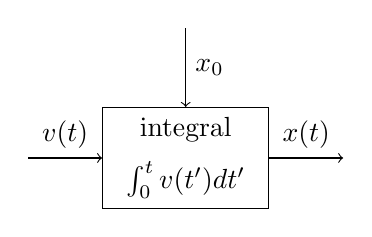
\begin{tikzpicture}[node distance=2cm]
\node[signal function with state, minimum width=6em] (integral) {integral \nodepart{second} $\int_0^t v(t') dt'$};
\coordinate[left of=integral] (in);
\coordinate[right of=integral] (out);
\coordinate[above=1cm of integral] (opt);
\draw [->] (in) to node[auto] {$v(t)$} (integral);
\draw [->] (integral) to node[auto] {$x(t)$} (out);
\draw [->] (opt) to node[auto] {$x_0$} (integral);
\end{tikzpicture}
\end{figure}
\item Linear movement: \mintinline{haskell}{pos = speed >>> integral 0}
\item Free fall from 100m: \mintinline[breaklines]{haskell}{pos' = gravity >>> integral 0 >>> integral 100}
    \end{itemize}
    \end{frame}
\begin{frame}{Examples}{Intervals}
    \begin{itemize}
    \item \mintinline{haskell}{after :: HasTime s => Time -> SF s a b}
    \item \mintinline{haskell}{for :: HasTime s => Time -> SF s a b}
    \item Game time-out after 60s, then game over for 10s
    \mint{haskell}{after 60 >>> for 10 >>> gameOver}
    \end{itemize}    
\end{frame}

\begin{frame}[fragile]{Examples}{Switching}
    \begin{itemize}
    \item \mintinline{haskell}{(-->) :: SF s a b -> SF s a b -> SF s a b}
    \item \mintinline{haskell}{f = f1 --> f2}:
        \begin{itemize}
        \item f1 produces $\Rightarrow$ f = f1
        \item f1 inhibits once $\Rightarrow$ f = f2
        \end{itemize}
    \item Elastic collision:
    \mint[breaklines]{haskell}{pos = (when (< wallPosition) (speed >>> integral 0) --> (speed >>> arr negate >>> integral wallPosition)}
    \end{itemize}
\end{frame}
    
\section{A functional game}
\begin{frame}{Introduction of our functional Game}
\centering\includegraphics[width=0.6\paperwidth, height=0.6\paperheight]{pong}
\end{frame}

\begin{frame}{Elm's Architecture}
\begin{columns}[T]
    \begin{column}{0.2\textwidth}
    \begin{itemize}
    \item<+-> Input
    \item<+-> Model
    \item<+-> Update
    \item<+-> View
    \end{itemize}
    \end{column}
    \hfill
    \begin{column}{0.8\textwidth}
    \begin{figure}[ht]
        \centering
            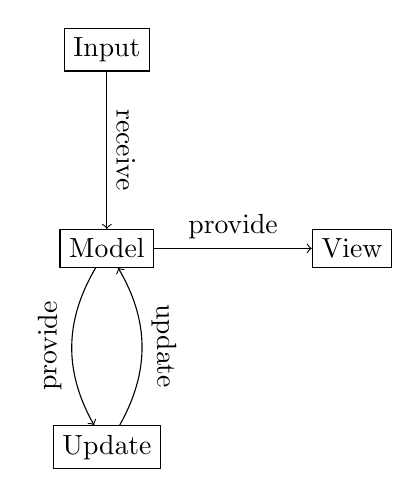
\begin{tikzpicture}
            \uncover<1->{\node[rectangle,draw] (input) {Input};}
            \uncover<2->{\node[rectangle,draw,below =2cm of input] (model) {Model};}
            \uncover<2->{\path[->, every node/.style={sloped,anchor=south,auto=false}]
            (input) edge  node {receive} (model);}
            \uncover<3->{\node[rectangle,draw,below =2cm of model] (update) {Update};}
            \uncover<3->{\path[->, every node/.style={sloped,anchor=south,auto=false}]
            (model) edge[bend right] node {provide} (update)
            (update) edge[bend right] node {update} (model);}
            \uncover<4->{\node[rectangle,draw,right =2cm of model] (view) {View};}
            \uncover<4->{\path[->, every node/.style={sloped,anchor=south,auto=false}]
            (model) edge node {provide} (view);}
            \end{tikzpicture}
    \end{figure}
    \end{column}
\end{columns}
\end{frame}

\section{Summary}
\begin{frame}{Summary}
\setbeamercovered{transparent}
\begin{itemize}
    \item<1> FRP
    \item<2> Implementation
    \item<3> Functional paradigm
\end{itemize}
\end{frame}

\begin{frame}{Outline}
\tableofcontents
% You might wish to add the option [pausesections]
\end{frame}

\setbeamertemplate{bibliography item}[triangle]
\begin{frame}[allowframebreaks]{References}
    \raggedright
    \nocite{Berntsen2014-game-systems-haskell}
    \nocite{hudak2003arrows}
    \nocite{Elliott2009-push-pull-frp}
    \nocite{elm-making-pong}
    \nocite{haskell-wiki-netwire}
    \bibliographystyle{plain}
    \bibliography{references}
\end{frame}


\end{document}